\documentclass[letterpaper,man,natbib]{apa6}  %Leave this stuff alone

\usepackage[english]{babel}
\usepackage[utf8x]{inputenc}
\usepackage{amsmath}
\usepackage{graphicx}
\usepackage{booktabs}
\usepackage[export]{adjustbox}

% dashed line (https://tex.stackexchange.com/questions/112343/beautiful-table-samples)
\usepackage{array}
\usepackage{arydshln}
\setlength\dashlinedash{0.2pt}
\setlength\dashlinegap{1.5pt}
\setlength\arrayrulewidth{0.3pt}

\title{Bifactor models of the `Maltreatment and Abuse Chronology of Exposure' (MACE) Scale}
\shorttitle{Bifactor models of MACE}
\author{Samuel Zorowitz$^1$, Lauri Tuominen$^{2}$}
\affiliation{$^1$Princeton Neuroscience Institute, Princeton University, USA\\$^2$The Royal’s Institute of Mental Health Research, University of Ottawa, Canada}

\abstract{Your abstract here.}

\begin{document}
\maketitle

\section{Introduction}

% "Happy families are all alike; every unhappy family is unhappy in its own way." – Leo Tolstoy.\break

Childhood maltreatment is a common experience for children across the world \citep{stoltenborgh2015prevalence}. It leads to an array of poor outcomes later in life, including the onset of mental illness \citep{macmillan2001childhood, green2010childhood, kessler2010childhood}, adverse effects on cognitive functioning \citep{kavanaugh2017neurocognitive, r2018common, su2019does}, and poorer physical health \citep{wegman2009meta, widom2012prospective, goodwin2004association}. Furthermore, childhood maltreatment predicts worse treatment outcomes across a variety of psychiatric disorders \citep{nanni2012childhood, thomas2019childhood, schuckher2019history}. As such, assessment of childhood maltreatment in a reliable and valid manner is important research goal in order to refine our understanding of the link between maltreatment and health outcomes; augment treatment strategies for victims of childhood maltreatment; and ultimately design interventions to prevent maltreatment in the first place. 

Many measures of childhood abuse and maltreatment have been developed \citep{saini2019systematic}. One recently introduced measure, the Maltreatment and Abuse Chronology of Exposure (MACE) scale \citep{teicher2015maltreatment}, has a number of notable advantages. The MACE is a 52-item self-report questionnaire of childhood maltreatment that assays 10 unique types of maltreatment. Six of these (i.e. parental physical maltreatment, parental non-verbal emotional abuse, parental verbal abuse, sexual abuse, physical neglect, emotional neglect) share overlap with other common measures of abuse (e.g. CTQ \citep{bernstein1998childhood} ); the remaining four solicit additional information on peer abuse, and witnessing violence at home. A number of previous scales were reviewed to select candidate items for the MACE. Item response theory and Rasch model were then used to for final selection of items for each 10 subscales. The MACE also measures detailed information on timing of exposure, which is critical for investigating how the onset of abuse shapes trajectories of development. Designed under the cumulative risk framework \citep{evans2013cumulative}, the MACE provides an overall severity score and multiplicity score (number of types of maltreatment experienced) with good test-retest reliability, convergent validity, and external validity.

More recently, there have been calls to move away from cumulative risk approach \citep{evans2013cumulative} --- which focuses on the number of adverse experiences, but does not distinguish between distinct types of environmental experience --- towards a dimensional approach, which emphasizes how specific types of maltreatment uniquely shape psycho-biological developmental trajectories \citep{mclaughlin2016beyond, belsky2012beyond}. As such, research groups have begun to use the MACE in other ways. Some groups have studied the unique contributions of all 10 subscales to psychopathology \citep{schalinski2015type, gerke2018childhood, schalinski2019early}. Following the threat-deprivation dimensional model \citep{mclaughlin2014childhood}, others have made composite indices of threat and deprivation using the MACE items measuring abuse and neglect, respectively \citep{schalinski2018defining, schalinski2019environmental, teicher2018differential}.

However, a critical challenge in measuring childhood maltreatment is the high co-occurrence of multiple types of abuse and neglect experiences; that is, children experiencing maltreatment are likely to be exposed to two or more types of maltreatment \citep{green2010childhood, mclaughlin2012childhood, marques2021risk, mersky2017rethinking}. For example, virtually all severely maltreated children report emotional abuse \citep{mcgee1995measurement}. As a consequence, isolating the unique contribution of a specific type of maltreatment (e.g. emotional neglect) to the risk of developing some outcome (e.g. depression) is difficult insofar that any one type of adversity is likely confounded with general maltreatment. Concretely, this means that researchers attempting to study the effects of particular types of maltreatment using subscale scores (e.g. emotional neglect from the MACE scale) should take pains to ensure that those measures largely reflect a construct unique from general maltreatment, as represented by the total score.

Bifactor models, a group of confirmatory factor analyses, are well-suited for addressing this issue \citep{bornovalova2020appropriate}. Bifactor models specify that the covariance among the items can be accounted for by a latent general factor, reflecting common variance among all items, and a set of latent specific factors, reflecting additional common variance for subsets of items \citep{Reise2012-ql}. Crucially bifactor models can be used to calculate model-based reliability statistics, e.g. the omega-hierarchical ($\omega_h$) and omega-subscale ($\omega_s$) indices, which respectively measure the proportion of variance in the total and subscale scores attributable to the general factor and specific factors \citep{reise2013applying, rodriguez2016evaluating}. Applied to MACE scale, these indices can guide researchers as to whether subscale scores for particular types of maltreatment are interpretable as such, or if they instead largely reflect general maltreatment. 
% summary of paper paragraph tk


% The bifactor model hypothesizes a general factor, onto which all items load, and a series of orthogonal (uncorrelated) skill-specific grouping factors
\section{Methods}

\subsection{Participants}

The participants in the current study (N=1633 total) belonged to one of two samples. The first sample of participants (N=1051) are from the original development of the MACE scale \citep{teicher2015maltreatment}. The full recruitment details for this sample have been reported elsewhere \citep{teicher2015maltreatment}. Briefly, these participants were recruited from the greater Boston area between 2010 and 2013. Inclusion criteria included being medically healthy, unmedicated, and between 18–25 years of age.  This sample will hereafter be referred to as the \textit{original} sample. 

The second sample of participants (N=687) were recruited from the Prolific Academic platform (\url{https://www.prolific.co}) to participate in an online experiment in August -- October, 2021. Of these, N=582 were retained for analysis (see Exclusion Criteria below). Participants were eligible for participation if they were 18 years or older and currently resided in the United States or Canada. Participants received monetary compensation for their time (rate: \$12 USD/hr). This study was approved by the Institutional Review Board of the University of Ottawa (protocol ID: 2021003), and all participants provided informed consent. This sample will hereafter be referred to as the \textit{replication} sample. 

In both the original and replication samples, the majority of participants identified as women (original: male = 381, female = 670; replication: male = 258, female = 310, nonbinary or other = 9, rather not say = 5). The original sample is comprised of proportionally more woman than the replication sample ($z = 4.142, p < 0.001$). On average, participants in the original sample were younger than participants in the replication sample ($M_1 = 23.1$ yrs, $M_2 = 30.2$ yrs, $t = -19.313, p < 0.001$). Finally, the majority of participants in both sample identified as Caucasian or white (original: 76.7\%; replication: 75.8\%). The proportion of participants identifying as white were not different across samples ($z = 0.417$, $p = 0.677$). 

\subsection{Measures}

All participants completed the 52-item version of the MACE scale \citep{teicher2015maltreatment}. The scale is a retrospective measure of the severity and timing of exposure to 10 types of childhood maltreatment. For each item, participants endorse whether they ever experienced a particular event during childhood (e.g. ``Parents or guardians intentionally pushed, grabbed, shoved, slapped, pinched, punched or kicked you'') and, if so, at what ages (up to age 18). Here we only analyze the binary endorsement responses (Yes = 1, No = 0) and not the chronology data. Six of the 52-items --- evenly divided between the emotional and physical neglect subscales --- are positively valenced (e.g. ``One or more individuals in your family helped you feel important or special'') and reverse-scored. For these items we follow the scoring convention set by \cite{teicher2015maltreatment}: a score of 1 is assigned to a response only in the absence of a positive event for all 18 years of childhood. This is in contrast to the remaining 46 items in the scale, where a score of 1 is assigned to a response if maltreatment or abuse occurred in at least one year of childhood.

In both the original and replication samples, participants completed a number of additional self-report symptom measures. We do not include these in our analyses and we will therefore not discuss these measures further in the main text. For completeness, we report these secondary self-report measures in the Supplementary Materials. 

\subsection{Exclusion criteria}

To ensure data quality in the replication sample, we relied on attention checks embedded in the self-report measures to identify and remove participants engaging in careless or insufficient effort responding \citep{zorowitz2021inattentive}. The data from N=64 (9.9\%)  participants in the replication sample were excluded for failing one or more of these attention checks, leaving the data from N=582 participants for analysis.

\subsection{Differential item functioning}

Prior to analysis, we investigated whether it was appropriate to combine response data from the original and replication samples. We first compared maltreatment endorsement rates for each item across samples. The Spearman-rank correlation of endorsement rates across samples was large ($\rho$ = 0.951, p < 0.001), indicating excellent correspondence in the relative prevalence of childhood maltreatment across samples. When we compare the distribution of person-level sum scores across samples,  however, we found that the number of maltreatment exposures was greater on average in the replication sample than in the original sample ($p_1$ = 0.185, $p_2$ = 0.219, $t$ = -4.611, p < 0.001). 

A mean shift in overall endorsement rates is not necessarily an indication that measurement invariance has been violated. One possibility is simply that participants in the replication sample had simply experienced more childhood maltreatment than participants in the original sample. A second possibility is that the differences in the demographic composition of the two samples (e.g. gender, age) moderate the differences in endorsement rates. To investigate these possibilities, we tested for uniform differential item functioning (DIF) using logistic regression \citep{rogers1993comparison}, in which a participant's endorsement response for an item was predicted by their rest score (i.e. their sum score for all other items), sample membership, gender, and age. 

Using the cutoffs recommended by \cite{hidalgo2014binary}, we identified 11 of 52 items on the MACE that exhibited large DIF by study (Figure S1). Interestingly these included all six of the reverse-scored items. We also found an additional 11 items that exhibited large DIF by gender (Figure S2). Five of these items concerned sexual abuse (endorsed by more women than men), and another five concerned peer physical abuse (endorsed by more men than women). We identified no items that exhibited large DIF by age. Given the number of items exhibiting DIF by sample membership, we elected to model each sample separately.

\subsection{Response dependency}

The MACE scale contains 12 sets of two to three items with response dependencies (Table S1). Some item sets share a structural dependency, where a response to one item logically requires or strongly implies a response on a second. For example, a person endorsing item 8 (``Parents or guardians hit you so hard that you received medical attention'') is all but certain to endorse item 7 (``Parents or guardians hit you so hard that it left marks for more than a few minutes''). Other item sets are characterized by redundancy dependency, where the same question is essentially asked twice using slightly different language. One such example is item 36 (``Peers forced you to engage in sexual activity against your will'') and 37 (``Peers forced you to do things sexually that you did not want to do``). 

For the current analyses, we were concerned about response dependence for two reasons. First, response dependence can inflate estimates of item discrimination parameters, thereby making items appear more informative than they actually are \citep{marais2008formalizing}. Second, in the context of bifactor models, specific factors may become contaminated by dependent items thereby making them appear more reliable than they actually are \citep{reise2013applying}. Following \cite{marais2008formalizing}, we therefore converted each set of dependent dichotomous items into a single polytomous item, thereby reducing the original 52-item MACE scale to 39 items.

\subsection{Confirmatory item factor models}

In order to evaluate the dimensionality of the MACE scale, we fit a series of four confirmatory item factor models to the endorsement data of each sample separately. The basis of each model was the The basis of each model was the graded response model for ordered polytomous data \citep{samejima1997graded}. The structure of each model is depicted in Figure \ref{fig:models}. The first model is a one-factor (undimensional) model whereby all items load onto a general maltreatment factor (Figure \ref{fig:models}a). The second is a bifactor model with a general maltreatment factor and 10 specific factors corresponding to each subscale of the MACE (Figure \ref{fig:models}b). 

The third model --- inspired by the deprivation-threat dimensional model \citep{mclaughlin2014childhood} --- is a bifactor S-1 model with a general maltreatment factor and one specific factor measuring neglect (Figure \ref{fig:models}c). We first attempted to fit this structure using a conventional bifactor model with two specific factors (i.e. threat, deprivation), but we observed vanishing factor loadings on the threat specific factor. Therefore, we instead utilized the bifactor S-1 model structure \citep{eid2017anomalous} where all of the threat (abuse) items comprise the general or reference factor, and the neglect items load onto both the general and specific factors. 

The fourth model attempts to provide a more parsimonious explanation of the MACE scale response data. We hypothesized items on the MACE can be summarized by overarching factors: maltreatment by adults in the home and maltreatment by peers. We also propose including a methods factor to account for unexplained variance in endorsements specific to the reverse-scored items. Thus, we tested a bifactor S-1 model with a general maltreatment factor and two specific factors (i.e. peer victimization, reverse-scoring; Figure \ref{fig:models}d). Similar to Model 3, initial fits of this structure using a conventional bifactor model with three specific factors resulted in vanishing factor loadings on the household abuse specific factor.

All the confirmatory item factor models were estimated within a Bayesian framework using Hamiltonian Monte Carlo as implemented in Stan (v2.26; \citealt{carpenter2017stan}). For all models, four separate chains with randomized start values each took 3,000 samples from the posterior. The first 2,000 samples from each chain were discarded, so that 4,000 post-warmup samples from the posterior were retained. The $\hat{R}$ values for all parameters were less than 1.01, indicating acceptable convergence between chains, and there were no divergent transitions in any chain. 

\subsection{Goodness of fit \& model comparison}

We relied on several indices to evaluate the fit of the models to the data. First we calculated three traditional goodness-of-fit statistics using the ordinal $M_2$ statistic \citep{cai2013limited, maydeu2013goodness}, which is asymptotically $\chi^2$-distributed with $\kappa − \nu$ degrees of freedom ($df$), where $\kappa$ is the number of reduced first- and second-order marginal residuals (i.e. $\kappa = n(n + 1)/2$ for $n$ items) and $\nu$ denotes the number of free parameters. (To improve the stability of the $M_2$, the polytomous items were binarized, corresponding to no versus any endorsement of maltreatment.)  Based on the $M_2$ statistic, we computed the root mean square error of approximation ($\text{RMSEA}_2$), comparative fit index (CFI), and Tucker-Lewis index (TLI). Following convention \citep{hu1999cutoff}, relatively good fit is indicated by the following indices: RMSEA < 0.06, CFI > 0.95, and TLI > 0.95. 

Given the questionable utility of SEM-based fit indices for item response theory applications (e.g. \citealt{reise2014evaluating}), we calculated two additional fit indices. First, we relied on posterior predictive model checking and a $\chi^2_{NC}$ discrepancy measure based on the total score distribution \citep{sinharay2006posterior}. This index compares the observed and expected proportion of participants who endorse maltreatment at each sum-score level. To detect local dependence, we calculated Yen's $Q_3$ statistic for each pair of items \citep{yen1984effects}. Following \cite{christensen2017critical}, we calculated the critical $Q_3$-value (i.e. the value above which local dependence is indicated) for each model and sample. Specifically, for each model and sample, we simulated 1000 locally-independent response datasets using the posterior distribution of item and ability parameters. We then recorded maximum $Q_3$ value per simulated dataset. The critical $Q_3$-value (per sample and dataset) was defined as the 99th percentile of the max $Q_3$ values.

Finally, the goodness-of-fit of the models was compared using Bayesian leave-one out cross-validation (LOO-CV; \citealt{vehtari2017practical}). The LOO-CV measure quantifies the discrepancy between the model and the data while taking into account model complexity. Here LOO-CV values are presented in deviance scale, such that smaller values indicate better fit.

\subsection{Reliability indices}

To evaluate the reliability of the MACE total and subscale scores, we calculated on several model-based reliability indices using the standardized factor loadings from the bifactor models. First, we calculated coefficient omega ($\omega$; \citealt{mcdonald1999test}), which quantifies the proportion of reliable score variance attributable to all factors (i.e. group and specific factors). Next we calculated the coefficient omega hierarchical ($\omega_h$) and coefficient omega subscale ($\omega_s$; \citealt{reise2013applying, rodriguez2016evaluating}). The $\omega_h$ index quantifies the fraction of variance in total scores that can be attributed to the individual differences on the general factor. By contrast, the $\omega_s$ index quantifies the fraction of variance in a subscale score that can be attributed to individual differences on a specific factor after controlling for the general factor. The $\omega_h$/$\omega_s$ values facilitate interpretation of the total and subscale scores. Values of $\omega_h$ approaching 1 indicate the general factor is the most dominant source of reliable variance in a total score. When $\omega_h$ is greater than 0.80, the total score on the scale may be considered essentially unidimensional \citep{rodriguez2016applying}. Similarly, values of $\omega_s$ approaching 1 increasingly indicate that individual differences on a subscale score reflect a specific factor and not the general factor. \cite{canivez2016bifactor} suggests that an acceptable $\omega_s$ value is 0.50 and that >0.70 is desirable. In contrast, $\omega_s$ values substantially smaller than 0.50 prevent meaningful interpretation of a subscale as reflecting a specific factor \citep{gignac2013bifactor}. 

In order to assess the unidimensionality of the MACE scale, we also calculated for each bifactor model and sample the explained common variance (ECV; \citealt{sijtsma2009use}) and the percent uncontaminated correlations (PUC; \citealt{reise2013multidimensionality}). The ECV is the ratio of the variance explained by the general factor divided by the total common variance of a scale, and thus quantifies the contribution of the general factor relative to the specific factors. As ECV values approach 1, general factor loadings are increasingly expected to resemble those that would be obtained by a one-dimensional model; ECV values greater than 0.70 are often indicative of essential unidimensionality \citep{rodriguez2016applying}. The PUC --- which quantifies how many inter-item correlations are accounted for only by the general factor --- is an important moderator of the ECV. When the PUC increases, the ECV is less important for evaluating the risk of bias when fitting a unidimensional model to data with a latent bifactor structure; when PUC is greater than 0.80, there is a low risk of bias when a multidimensional scale is treated as unidimensional \citep{reise2013multidimensionality}. As an additional check, we calculated for each bifactor model the relative parameter bias, or the difference between an item's loading in the unidimensional  model and its corresponding general factor loading the bifactor, divided by the general factor loading in the bifactor. Parameter bias less than 10–15\% is acceptable \citep{muthen1987structural}.

Though of secondary interest, we also calculated the H index to assess the construct construct replicability of each factor \citep{hancock2001rethinking}. The H index is an estimate of how well a set of items represents a latent variable. Larger H values (e.g. $> 0.70$) indicate a well-defined latent variable, with factor loadings more likely to be stable across studies; conversely, low H values suggest a poorly defined latent variable, where the pattern of factor loadings are liable to change across studies \citep{hancock2001rethinking}.

\subsection{Exploratory factor analysis}

In addition to confirmatory factor analysis, we also performed exploratory factor analysis (EFA) on the endorsement data from both samples to see what factor structure would emerge with no \emph{a priori} restrictions \citep{schmitt2018selecting}. We elected to extract two- and three-factor solutions based to match the number of factors in the two bifactor S-1 models. That is, we wanted to see if a two-factor solution would resemble threat and deprivation factors; and if a three-factor solution would resemble family maltreatment, peer victimization, and reverse-scoring factors. 

EFA was performed using the \textit{lavaan} (v0.6.11; \citealt{lavaan}) package available in R. Factors were extracted using the geomin \citep{yates1987multivariate} and cf-quartimax rotation criteria \citep{crawford1970general}, which were selected in order to extract simple factor structures with few cross-loadings. We used two rotation criteria in order to examine the generalizability of the factor solutions across oblique and orthogonal rotations. 

\section{Results}

\subsection{Goodness-of-fit \& model comparison}

The fit indices for each model and sample are summarized in Table \ref{table:diagnostics}. According to the traditional indices, we found all four models provided an acceptable fit to the response data. Across samples, all the models had RMSEA values < 0.06 and the majority exhibited CFI and TLI values > 0.95. The exception were models 1 and 3 in the original sample, which exhibited acceptable fits (CFI and TFI values > 0.90). In general, model fits were better for the replication sample data than for the original sample. Furthermore none of the posterior predictive p-values corresponding to the $\chi^2_{NC}$ discrepancy measure exceeded the critical value, indicating that all models were sufficiently able to replicate the sum score distribution for each sample. 

Next we inspected the $Q_3$ indices for evidence of local dependence. For all models and samples, the maximum observed $Q_3$ index was greater than the 99\% percentile critical value indicating the presence of local dependence. To understand the extent of the local dependence, we visualized the $Q_3$ values for item pairs exceeding the critical value for each model and sample (Figure S3). For both samples the unidimensional model exhibited many item pairs with local dependence, predominantly among the peer victimization and reverse-scored items, suggesting possible underfactorization. By comparison, the remaining models exhibited far fewer locally dependent item pairs, the majority of which were easy to understand. For example, the large $Q_3$ value for item 17 (``Parents made inappropriate sexual comments or suggestions to your sibling or stepsibling'') and item 18 (``Parents touched or fondled your sibling or stepsibling in a sexual way'') is easily understood as surface local dependence. Regardless, the estimated item discrimination parameters for all models and samples seldom exceeded the usual range (i.e. $\alpha \leq 4$) suggesting that whatever local dependence was present is exerting minimal bias on parameter estimates \citep{edwards2018diagnostic}. Thus, we conclude that all of the models provide at least acceptable fits to the response data from both samples.

The results of the model comparison are also summarized in Table \ref{table:diagnostics}. In both the original and replication datasets, models 2 and 4 exhibited better fit to the data than models 1 and 3. Between models 2 and 4, the former provided a numerically better fit in the original sample ($\Delta$ LOO = 7.9, se = 56.3) but a worse fit in the replication sample ($\Delta$ LOO = -24.0, se = 52.0). The differences in LOO-CV values are both within four standard errors of the mean, however, indicating only weak predictive improvements \citep{vehtari2022cv}. Thus, the model comparison suggests that models 2 and 4 yield approximately equal fits to the data, which is noteworthy insofar that model 4 assumes a much simpler and parsimonious factor structure of the MACE scale.

\subsection{Confirmatory item factor models}

The standardized factor loadings from the unidimensional model fit to the original and replication datasets are are summarized in the first column of Figure \ref{fig:loadings_original} and Figure \ref{fig:loadings_online} respectively.

\subsection{Model 1: Unidimensional model}

To begin we fit a unidimensional model to the MACE response data, in which all items load onto a single general maltreatment factor (Figure 1a). In the original dataset, the item discrimination parameters were between 0.506 and and 2.944, with an average value of 1.357 (95\% HDI = 1.295 -- 1.414). For the replication dataset, item discrimination ranged between 0.657 and 2.407 with an average value of  1.349 (95\% HDI = 1.272 -- 1.422). Across datasets, all but one item exhibited medium ($\alpha \in$ 0.65 -- 1.34) to high ($\alpha \in$ 1.35 -- 1.69) levels of discrimination \citep{baker2017basics}. Differences in item discrimination estimates between datasets were marginal (RMSE = 0.038, 95\% HDI = 0.014 -- 0.068), indicating consistency of discrimination across samples. 

In the original dataset, factor loadings ranged between 0.279 and 0.864, with an average value of 0.597 (95\% HDI = 0.579 -- 0.614). Similarly, in the replication dataset, factor loadings ranged between 0.359 and 0.814 with an average value of 0.600 (95\% HDI = 0.578 -- 0.621). With the exception of item 42, all items across datasets exhibited consistent and moderate-to-large loadings on the unitary factor. In other words, all but one item appear to measure, at least in part, general maltreatment. 

\subsection{Model 2: Bifactor model with 10 specific factors}

The standardized factor loadings from the fit of the bifactor model to the original and replication datasets are are summarized in the second column of Figure \ref{fig:loadings_original} and Figure \ref{fig:loadings_online} respectively. For both datasets, the factor loadings on the general factor largely resembled those from the unidimensional models. The average magnitude of the factor loadings was 0.575 (95\% HDI = 0.556 -- 0.593) for the original dataset and 0.580 (95\% HDI = 0.560 -- 0.601) for the replication dataset. The relative parameter bias\footnote{The relative parameter bias is defined as the difference between an item’s loading in the unidimensional solution and its general factor  loading in the bifactor, divided by the general factor loading in the bifactor model.} was 2.1\% for the original dataset and 2.7\% in the replication dataset, indicating little bias in the factor loadings in a unidimensional solution due to multidimensionality.  

In contrast loadings on the specific factors were predominantly small-to-moderate in magnitude, and seldom exceeded loadings on the general factor. In the original dataset, specific factor loadings ranged 0.014 to 0.797 with an average value of 0.313 (95\% HDI = 0.285 -- 0.341). For the replication dataset, the range was 0.043 to 0.698 with an average value of 0.343 (95\% HDI = 0.315 -- 0.369). Only items from the peer victimization subscales (i.e. PeerVA, PeerPA) had specific factor loadings of roughly equal or greater magnitude than those of general factor. 

Next we inspected the reliability of the MACE total score. The $\omega$ values indicated the total score had excellent reliability in both the original ($\omega$ = 0.963) and replication ($\omega$ = 0.965) datasets. Across datasets, the omega hierarchical values was 0.924 indicating that 96.0\% and 95.8\% of the reliable variance in total scores are attributable to general maltreatment. Moreover, the explained common variance values were 0.716 for the original dataset and 0.697 for the replication dataset. This indicates the presence of a strong general maltreatment factor in the dataset, and suggests MACE response data is largely undimensional. 

Next we inspected the reliability of the MACE subscale scores. The model-based reliability indices were variable in both the original (mean $\omega$ = 0.750, range = 0.590 -- 0.909) and replication (mean $\omega$ = 0.756, range = 0.595 -- 0.893) datasets, though most subscale scores exhibited adequate reliability. Crucially, the omega subscale were typically small in both the original (mean $\omega_s$ = 0.181, range = 0.027 -- 0.621) and (mean $\omega_s$ = 0.205, range = 0.037 -- 0.565) replication datasets. This indicates that most subscale scores contain little reliable variance apart from the general factor; that is, the majority of MACE subscales scores cannot be meaningfully interpreted as such. The only exception was for the peer verbal abuse subscale, where more than half the reliable variance in subscale scores were independent of general maltreatment (original = 70.7\%; replication = 66.2\%). These findings were echoed in the H index values, which were unacceptably small for all subscales across both datasets (with an exception again for the peer verbal abuse subscale).  

\subsection{Model 3: Bifactor S-1 model with one specific factor (neglect)}

As for the full bifactor model, the factor loadings on the threat-deprivation bifactor S-1 model resembled those from the unidimensional models. The average magnitude of the factor loadings was 0.575 (95\% HDI = 0.556 -- 0.593) for the original dataset and 0.580 (95\% HDI = 0.560 -- 0.601) for the replication dataset. The standardized factor loadings for the specific factor (i.e. deprivation) were on average [stats here]. The loadings, however, exhibited a striking pattern where only the reverse-scored items exhibited moderate loadings; the the remaining four items exhibited negligible loadings. That is, the "deprivation" factor appears to reflect a methods factor instead. 

Though the subscale reliability was adequate (original: $\omega$ = 0.877; replication: $\omega$ = 0.921), the omega subscale values indicated that neglect scores contained less than half reliable variance unique from the general factor (original: $\omega_h$ = 0.384; replication: $\omega_h$ = 0.375). Not only is the validity of the deprivation subscale questionable, but so too is its reliability.   

\subsection{Model 4: Bifactor S-1 with two specific factors (peer victimization, reverse-scoring)}


Again the standardized factor loadings on general factor of the parsimonious bifactor S-1 model resembled those from the unidimensional models. The average magnitude of the factor loadings was 0.575 (95\% HDI = 0.556 -- 0.593) for the original dataset and 0.580 (95\% HDI = 0.560 -- 0.601) for the replication dataset. Notably, the factor loadings of the peer victimization and methods factor were also moderate in magnitude and on average larger than those observed on the general factor, lending credence for their independence. 

In contrast, the peer victimization factor of the second bifactor S-1 model (Model 4) exhibited good subscore reliability in both datasets original: $\omega$ = 0.889; replication: $\omega$ = 0.868) and adequate omega subscale reliability (original: $\omega_h$ = 0.569; replication: $\omega_h$ = 0.493). In other words, more half of its reliable variance was unique from the general factor (original = 0.640; replication = 0.568). 

\subsection{Exploratory factor analysis}

The standardized factor loadings for the two- and three-factor solutions generated by the cf-quartimax rotation are summarized in Figure \ref{fig:efa}. (The corresponding factor loadings yielded by the geomin rotation were largely similar and are presented Figure S1.) In the two-factor solutions, two unique factor structures emerged by dataset. In the original dataset, there was a dominant household maltreatment factor and a secondary peer victimization factor. In contrast, the replication dataset exhibited a primary factor comprised of household and peer maltreatment, and a secondary reverse-scoring methods factor. 

In the three-factor solutions, the recovered factor structures were largely similar across datasets. There was a household maltreatment factor, a peer victimization factor, and a reverse-scoring methods factor. Of note, the sexual abuse items seemed to load more strongly on the peer victimization factor in the replication dataset than in the original dataset, warranting some caution in interpreting the stability of the factor structures. In sum, the structure of both the two- and three-factor EFA solutions resembled the bifactor S-1 model with specific peer victimization and reverse-scoring methods factors (Model 4), providing additional support for this model of covariation in childhood maltreatment. 

\section{Discussion}

%------------------------------------%
% Discussion: summary
%------------------------------------%

% essentially unidimensional, sans a smaller social factor

%------------------------------------%
% Discussion: previous factor models of maltreatment scales
%------------------------------------%

Our results are consistent with a number of other studies that have found a dominant general factor in measures of childhood maltreatment. Applying a bifactor model to the childhood trauma questionnaire, \cite{spinhoven2014childhood} identified a robust general maltreatment factor that explained away the majority of reliable variance in subscale scores (with the exception of sexual abuse). \cite{meinck2021factor} found similar results when investigating the bifactor structure of the International Child Abuse Screening Tool (ICAST). In a recent investigation of the adverse childhood experience (ACE) questionnaire, \cite{dobson2021latent} found that on average items loaded more strongly onto the general factor than onto their respective specific factors. Collectively these results echo the co-occurrence of types of childhood maltreatment across measurement tools. 

In turn, our results are worth interpreting in light of recent studies using MACE subscale scores to investigate the relationship between particular types of childhood maltreatment and various psychopathological or neurobiological outcomes. For example, recent studies have used the 10 MACE subscales to look at the relationship of particular types of childhood maltreatment to lifetime risk of depression \citep{gerke2018childhood}, dissociative symptoms in schizophrenia \citep{schalinski2015type}, and cortisol concentration \citep{schalinski2019early}. Others have used the MACE to form indices of threat and deprivation to study... Our results indicate that, reflecting the cofrequency of maltreatment, most of the reliable variance in these subscale scores are attributable to general maltreatment and not any of the specific types of maltreatment intended to be assessed. Many of these studies attempt to bypass these issues by use of more sophisticated analytic techniques, such as random forest regression. One issue is that these methods are not necessarily protective against collinearity \citep{gregorutti2017correlation}. But this point belies the deeper problem that it is difficult to imagine how a researcher would make substantive sense of a study reporting differential correlates for total and subscale scores, given the redundancy, as well as the low reliability of the part of the subscale not redundant with the total score. As such, results from these earlier studies should be interpreted with caution. As discussed above, general factor may account for most of the variance independent of the measurement tool. Thus, these issues may be prevalent throughout the childhood maltreatment research literature that has explored contributions of a single maltreatment type (e.g. emotional neglect) to an outcome.  
 
 In sum, bifactor models fit to MACE response data revealed the presence of a strong general maltreatment factor that explained the majority of variance in the response data. Moreover, an interrogation of subscale scores revealed these to be largely unreliable measures of specific types of maltreatment. In other words, MACE subscale scores predominantly reflect overall maltreatment and cannot be interpreted as unique measures of specific maltreatment. The sum total of these results further suggest the MACE is essentially unidimensional, reflecting general severity of maltreatment. 

 
%------------------------------------%
% Discussion: formative vs. reflective indicators
%------------------------------------%

% not clear to me this topic is relevant anymore

% These issues reflect a more fundamental question: whether to consider childhood maltreatment a formative or reflective variable \citep{bollen2011three}. On the one hand, maltreatment and adversity events define trauma exposure and can thus be understood as a formative variable; indeed others have argued that trauma events should be understood as formative \citep{netland2001assessment, layne2010unpacking}. On the other hand, certain types of maltreatment likely reflect a common generative process (e.g. parental style correlated neglect and physical abuse) \citep{hall2010measuring}. Childhood maltreatment may also be better understood as reflecting a general process in the context of retrospective recall, where psychological processes may shape the recall and reporting of childhood events \citep{dovran2013psychometric}. This issue is not merely semantic; it has important consequences for how we understand, measure, and interpret maltreatment data. 

%------------------------------------%
% Discussion: differential item functioning (gender, reverse-scoring, sample?)
%------------------------------------%

In both data sets, women endorsed more sexual abuse, and men reported more physical abuse by peers. These results are in line with previous studies showing that girls are more often victims of sexual abuse \citep{stoltenborgh2015prevalence}, whereas boys are more often victims of bullying, especially physical bullying \citep{scheithauer2006physical}. We also found evidence that a fifth of items in the MACE exhibited some differential item functioning across the two samples. That is, the response rate for XX, YY was higher in ... . These differences may be attributable to different populations (Boston vs. across Canada \& USA), recruitment (local advertisement vs. prolific.co), exclusion criteria (required to be healthy and unmedicated vs. none), generational effect (data collected in 2010-2013 vs. 2021), technical differences in the online assessment platform ("HIPAA-compliant online enrollment system" vs. website built specifically to collect MACE data with jspsych \citep{de2015jspsych}), or differences in excluding inattentive or careless responders (none vs. infrequency items \citep{zorowitz2021inattentive}). 


%------------------------------------%
% Discussion: peer victimization, bullying
%------------------------------------%

The best fitting model suggested that the MACE contains an independent peer victimization (bullying) factor comprised of items in the peer verbal abuse and peer physical abuse subscales. Correlation between the bullying factor and the general factor was moderate. In accordance, a previous report on two prospective cohorts estimated that around 40\% of children who were maltreated were also bullied \citep{lereya2015adult}. The authors of that study speculated that there may be common risk factors for childhood maltreatment and bullying such as family instability and poor social skills. On the other hand, the authors also hypothesized that maltreatment may make children more susceptible to bullying by, for instance, disrupting the child's ability to regulate emotions. Similar to childhood maltreatment by household members, bullying by peers is a common childhood experience \citep{world2020spotlight} and has detrimental effects on mental health independent of other types of childhood maltreatment \citep{singham2017concurrent, lereya2015adult}. Separating peer bullying as its own factor in the MACE may therefore offer a more granular view of the harmful childhood experiences of the responders. In the future, the peer bullying factor should be validated against other restrospective bullying measures such as the California Bullying Victimization Scale \citep{green2018initial}. Finally, the MACE does not assess cyberbullying which is an increasingly common form of bullying. 

%------------------------------------%
% limitations
%------------------------------------%

%------------------------------------%
% future directions: age data
%------------------------------------%

%------------------------------------%
% conclusions / recommendations
%------------------------------------%

\bibliography{main}

\begin{table}
\small
\centering
\begin{adjustbox}{center}
\begin{tabular}{ccccccccccr}
\toprule
Sample & Model & $\chi^2 (df)$ &  RMSEA & CFI & TLI & $\chi^2_{NC}$ (PPP) & $Q3_{\max}$ &  $Q3_{\text{crit}}$ & LOO-CV & \multicolumn{1}{c}{$\Delta$LOO (se)} \\
\midrule
Original & 1 &  1858 (702) &  0.040 &  0.927 &  0.923 &  0.051 (0.230) &  0.589 &  0.239 &  30967.2 &  1748.0 (76.7) \\
& 2 &  1373 (663) &  0.032 &  0.955 &  0.950 &  0.046 (0.356) &  0.573 &  0.300 &  29211.3 & \multicolumn{1}{c}{-} \\
& 3 &  1571 (692) &  0.035 &  0.944 &  0.940 &  0.051 (0.214) &  0.591 &  0.255 &  30531.1 &  1312.0 (68.0) \\
& 4 &  1253 (687) &  0.028 &  0.964 &  0.961 &  0.046 (0.346) &  0.591 &  0.279 &  29219.2 & 7.9 (56.3) \\
\midrule
Replication & 1 &  1086 (702) &  0.031 &  0.954 &  0.952 &  0.065 (0.629) &  0.513 &  0.250 &  19771.6 &  1089.3 (58.4) \\
& 2 &   956 (663) &  0.028 &  0.965 &  0.961 &  0.058 (0.766) &  0.456 &  0.310 &  18706.2 &    24.0 (52.0) \\
& 3 &   881 (692) &  0.022 &  0.977 &  0.976 &  0.062 (0.684) &  0.468 &  0.316 &  19177.7 &   495.5 (45.0) \\
& 4 &   842 (687) &  0.020 &  0.982 &  0.980 &  0.058 (0.756) &  0.437 &  0.318 &  18682.2 & \multicolumn{1}{c}{-} \\
\bottomrule
\end{tabular}
\end{adjustbox}
\captionsetup{width=1.1\textwidth}
\caption{\normalfont Fit statistics for the confirmatory factor models by sample. LOO-CV values are presented in deviance scale (i.e. smaller values indicate better fit). Abbreviations: RMSEA = root mean square error of approximation; CFI = comparative fit index; TLI = Tucker-Lewis index; PPP = posterior predictive p-value; $Q3_{\max}$ = maximum $Q_3$ value in the sample for the model; $Q3_{\text{crit}}$ = critical $Q_3$ value for the model; LOO-CV = leave-one-out cross-validation.}
\label{table:diagnostics}
\end{table}

\begin{table}
\centering
\begin{tabular*}{\textwidth}{crccccccccc}
\toprule
& & & \multicolumn{4}{c}{Original} & \multicolumn{4}{c}{Replication} \\
\cmidrule(lr){4-7}\cmidrule(lr){8-11}
Model & Subscale & PUC & ECV & $\omega$ & $\omega_{h/s}$ & H & ECV & $\omega$ & $\omega_{h/s}$ & H \\
\midrule
2 & General  &  0.912&0.716 &  0.963 &   0.924 &  0.964&0.697 &  0.965 &   0.924 &  0.961 \\
& VA       &       &      &  0.909 &   0.069 &  0.273&      &  0.893 &   0.162 &  0.478 \\
& PA       &       &      &  0.590 &   0.037 &  0.052&      &  0.595 &   0.148 &  0.194 \\
& NVEA     &       &      &  0.848 &   0.136 &  0.525&      &  0.827 &   0.117 &  0.424 \\
& SA       &       &      &  0.710 &   0.059 &  0.134&     &  0.749 &   0.290 &  0.452 \\
& EN       &       &      &  0.715 &   0.162 &  0.304&     &  0.874 &   0.203 &  0.542 \\
& PN       &       &      &  0.800 &   0.217 &  0.479&     &  0.812 &   0.114 &  0.284 \\
& WSV      &       &      &  0.695 &   0.027 &  0.053&     &  0.651 &   0.037 &  0.067 \\
& WIPV     &       &      &  0.655 &   0.146 &  0.197&      &  0.612 &   0.077 &  0.107 \\
& PeerVA   &       &      &  0.878 &   0.621 &  0.818&     &  0.853 &   0.565 &  0.766 \\
& PeerPA   &       &      &  0.699 &   0.335 &  0.443&     &  0.694 &   0.337 &  0.446 \\
\midrule
3 & General &  0.939&0.864 &  0.958 &   0.928 &  0.964&0.841 &  0.959 &   0.922 &  0.959 \\
& neglect &       &      &  0.877 &   0.384 &  0.766&      &  0.921 &   0.375 &  0.814 \\
\midrule
4 & General &  0.931&0.738 &  0.961 &   0.896 &  0.965&0.751 &  0.961 &   0.904 &  0.960 \\
& Peer    &       &      &  0.889 &   0.569 &  0.842&      &  0.868 &   0.493 &  0.781 \\
& Reverse &       &      &  0.839 &   0.584 &  0.739&     &  0.915 &   0.498 &  0.773 \\
\bottomrule
\end{tabular*}
\captionsetup{width=1.\textwidth}
\caption{\normalfont Model-based reliability indices for the three bifactor models. Abbreviations: VA = verbal abuse; PA = physical abuse; NVEA = nonverbal emotional abuse; SA = sexual abuse; EN = emotional neglect; PN = physical neglect; WSV = witnessing sibling violence; WIPV = witnessing inter-parental violence; PeerVA = peer verbal abuse; PeerPA = peer physical abuse; ECV = explained common variance.}
\label{table:reliability}
\end{table}

\begin{figure}
    \centering
    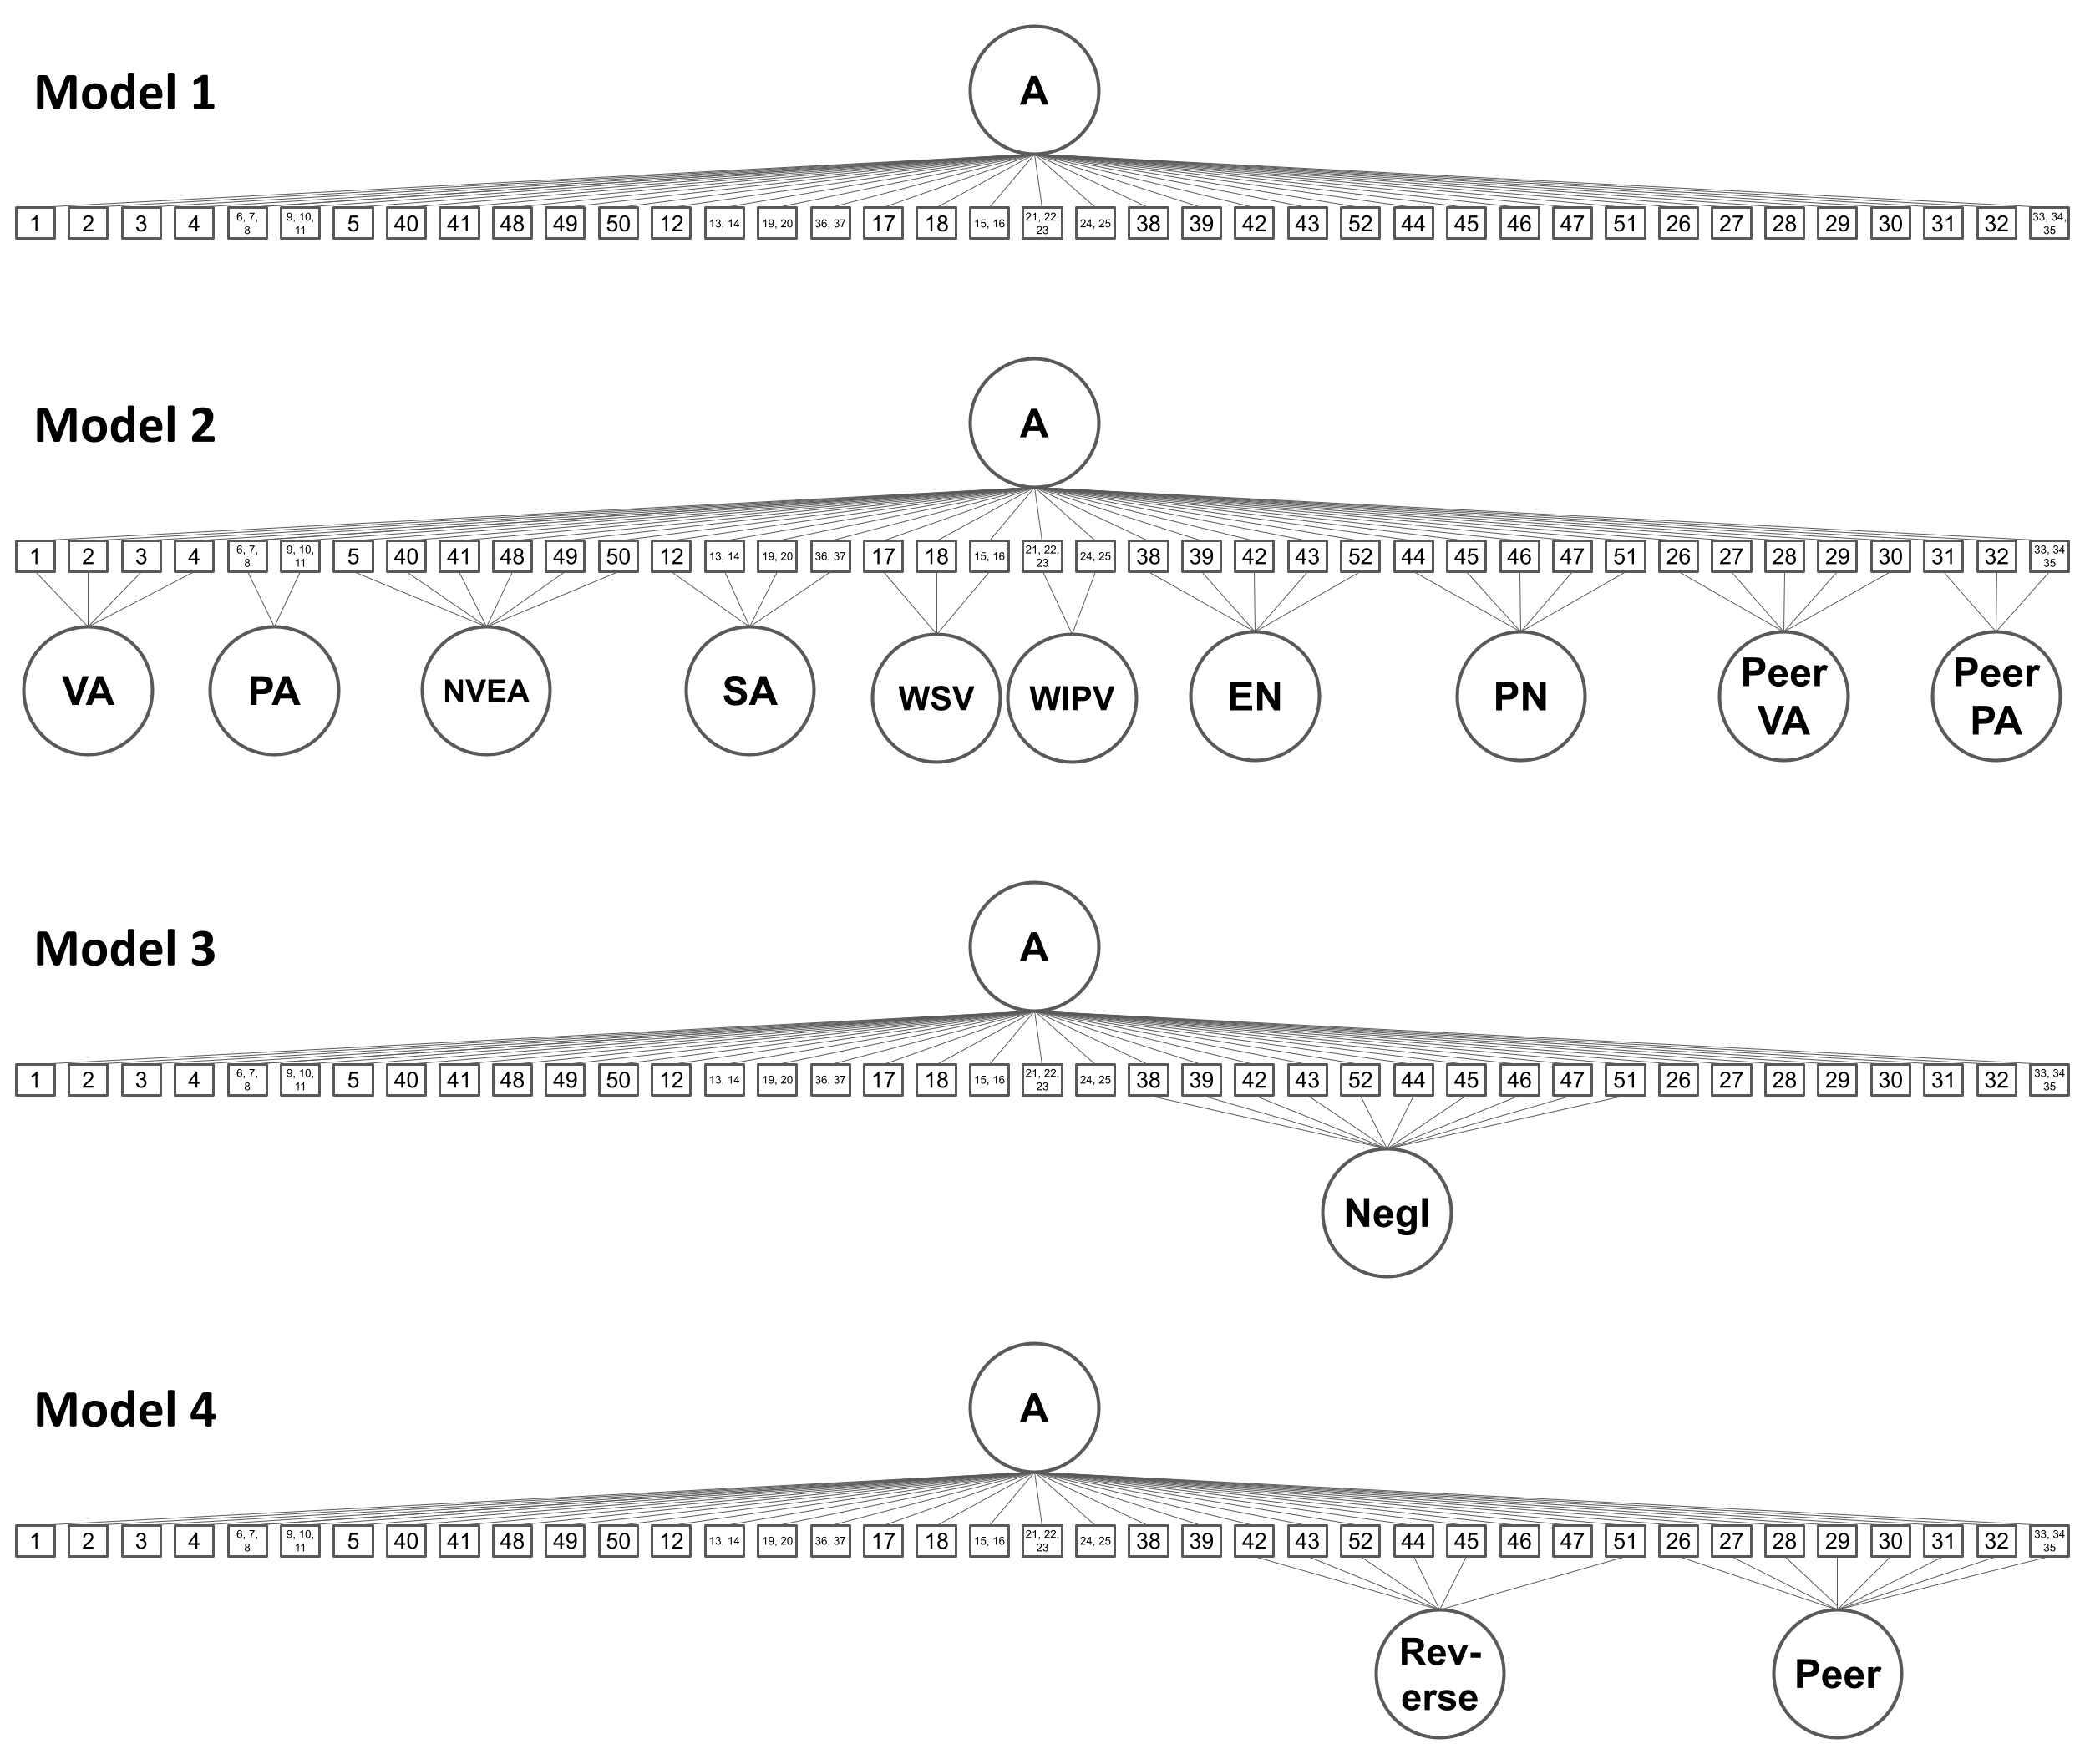
\includegraphics[width=1.1\textwidth,center]{figures/fig00.png}
    \caption{Caption}
    \label{fig:models}
\end{figure}

\begin{figure}
    \centering
    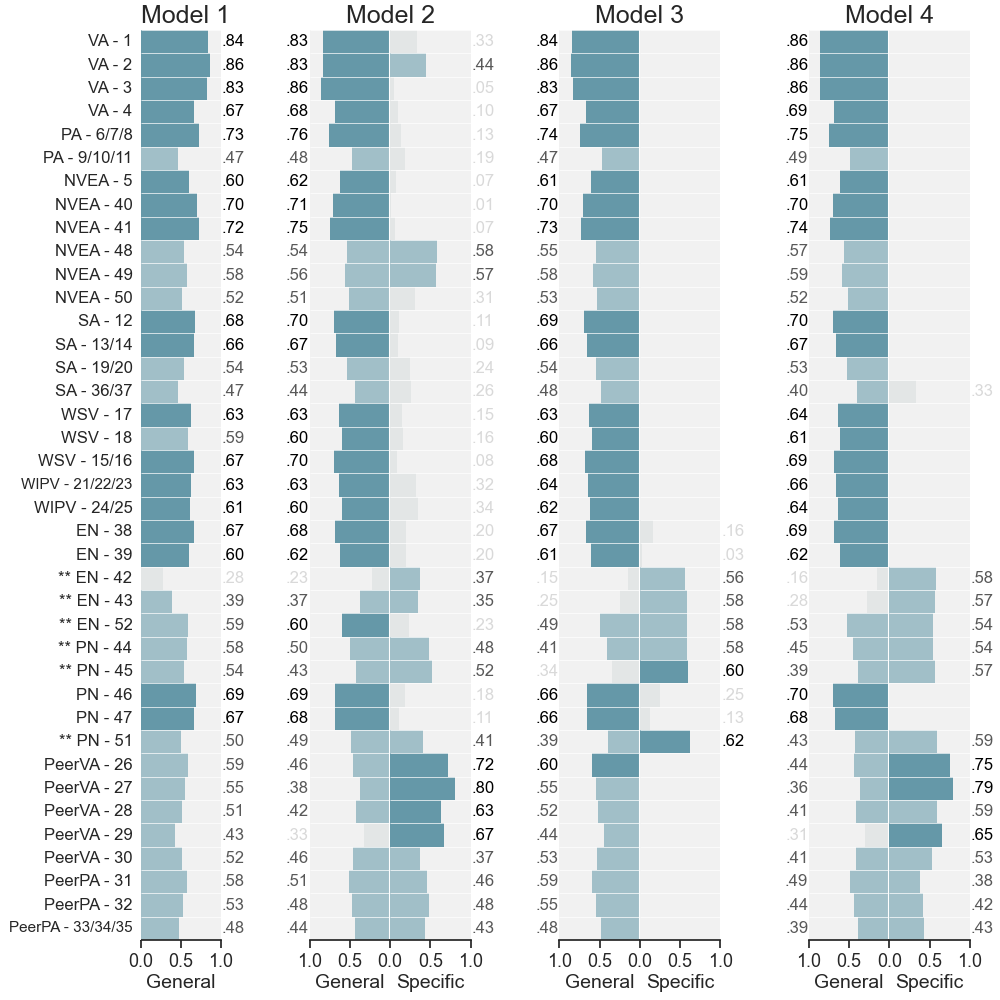
\includegraphics[width=1.1\textwidth,center]{figures/fig01.png}
    \caption{Standardized factor loadings from the four models estimated from the original dataset. VA = verbal abuse; PA = physical abuse; NVEA = nonverbal emotional abuse; SA = sexual abuse; WSV = witnessing sibling vioence; WIPV = witnessing inter-parental violence; EN = emotional neglect; PN = physical neglect; PeerVA = peer verbal abuse; PeerPA = peer physical abuse. ** Reverse-scored items.}
    \label{fig:loadings_original}
\end{figure}

\begin{figure}
    \centering
    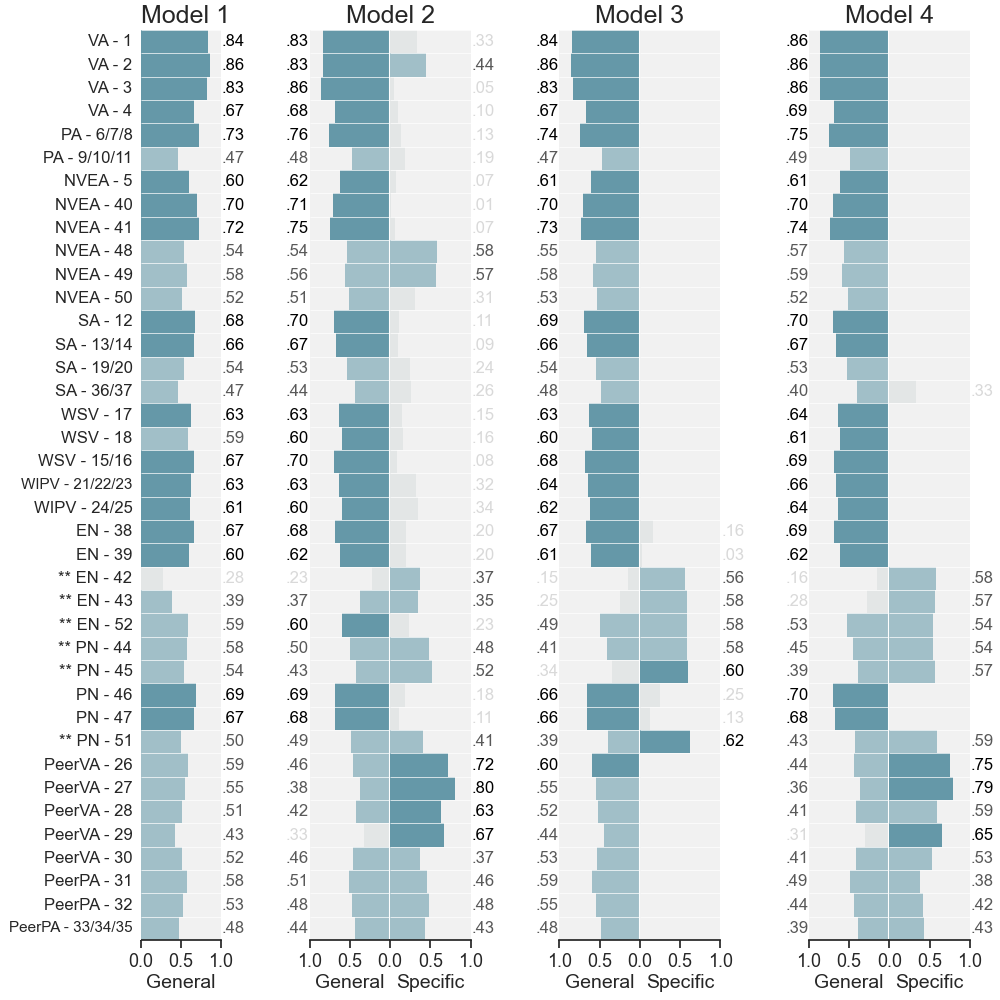
\includegraphics[width=1.1\textwidth,center]{figures/fig02.png}
    \caption{Standardized factor loadings from the four models estimated from the online dataset. VA = verbal abuse; PA = physical abuse; NVEA = nonverbal emotional abuse; SA = sexual abuse; WSV = witnessing sibling vioence; WIPV = witnessing inter-parental violence; EN = emotional neglect; PN = physical neglect; PeerVA = peer verbal abuse; PeerPA = peer physical abuse. ** Reverse-scored items.}
    \label{fig:loadings_online}
\end{figure}

\begin{figure}
    \centering
    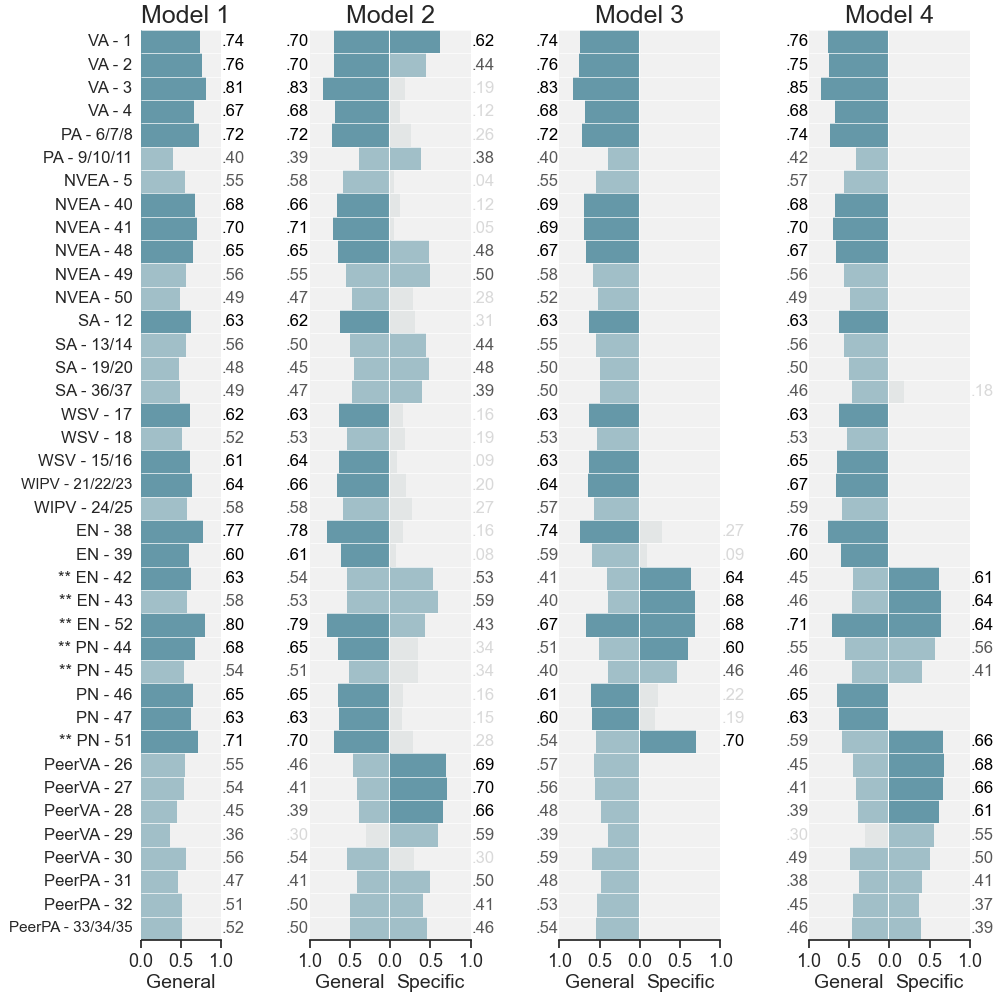
\includegraphics[width=1\textwidth,center]{figures/fig03.png}
    \caption{Caption}
    \label{fig:efa}
\end{figure}

\end{document}
